
%%%%%%%%%%%%%%%%
%%%%%%%%%%%%%%%%

\section{Biogeographic dating using DEC}

This analysis will jointly estimate phylogeny and biogeography.
One benefit is that the biogeographic analysis will intrinsically accommodate phylogenetic uncertainty.
Another is that paleogeographic evidence may provide information about the geological timing of speciation events in the phylogeny.
Finally, biogeographic data may lend support to certain phylogenetic relationships that have poor resolution otherwise.

Hawaiian silverswords are nested in a larger group of plants, the tarweeds.
Fossil pollen evidence indicates that tarweeds diversified during a period of aridification from 15--5 Ma in the western regions of North America (cite Baldwin papers).
Although the oldest Hawaiian island that silverswords inhabit is Kauai, it is possible that silverswords first colonized older islands in the Emperor Island chain that predate the formation of Kauai at about 5.1 Ma.

This makes traditional node-based biogeographic calibrations challenging, because it would require a strong assumption about when and how many times the oldest silversword lineages colonized Kauai.
Did silverswords colonize Kauai once directly from the California coast? Or did the colonize the younger islands multiple times from older islands in the chain? And did the event occur immediately after Kauai surfaced or much later? Because we cannot observe the timing and nature of this event directly, this process-based biogeographic dating approach does so through probabilistic inference.

\begin{figure}[!ht]
\centering
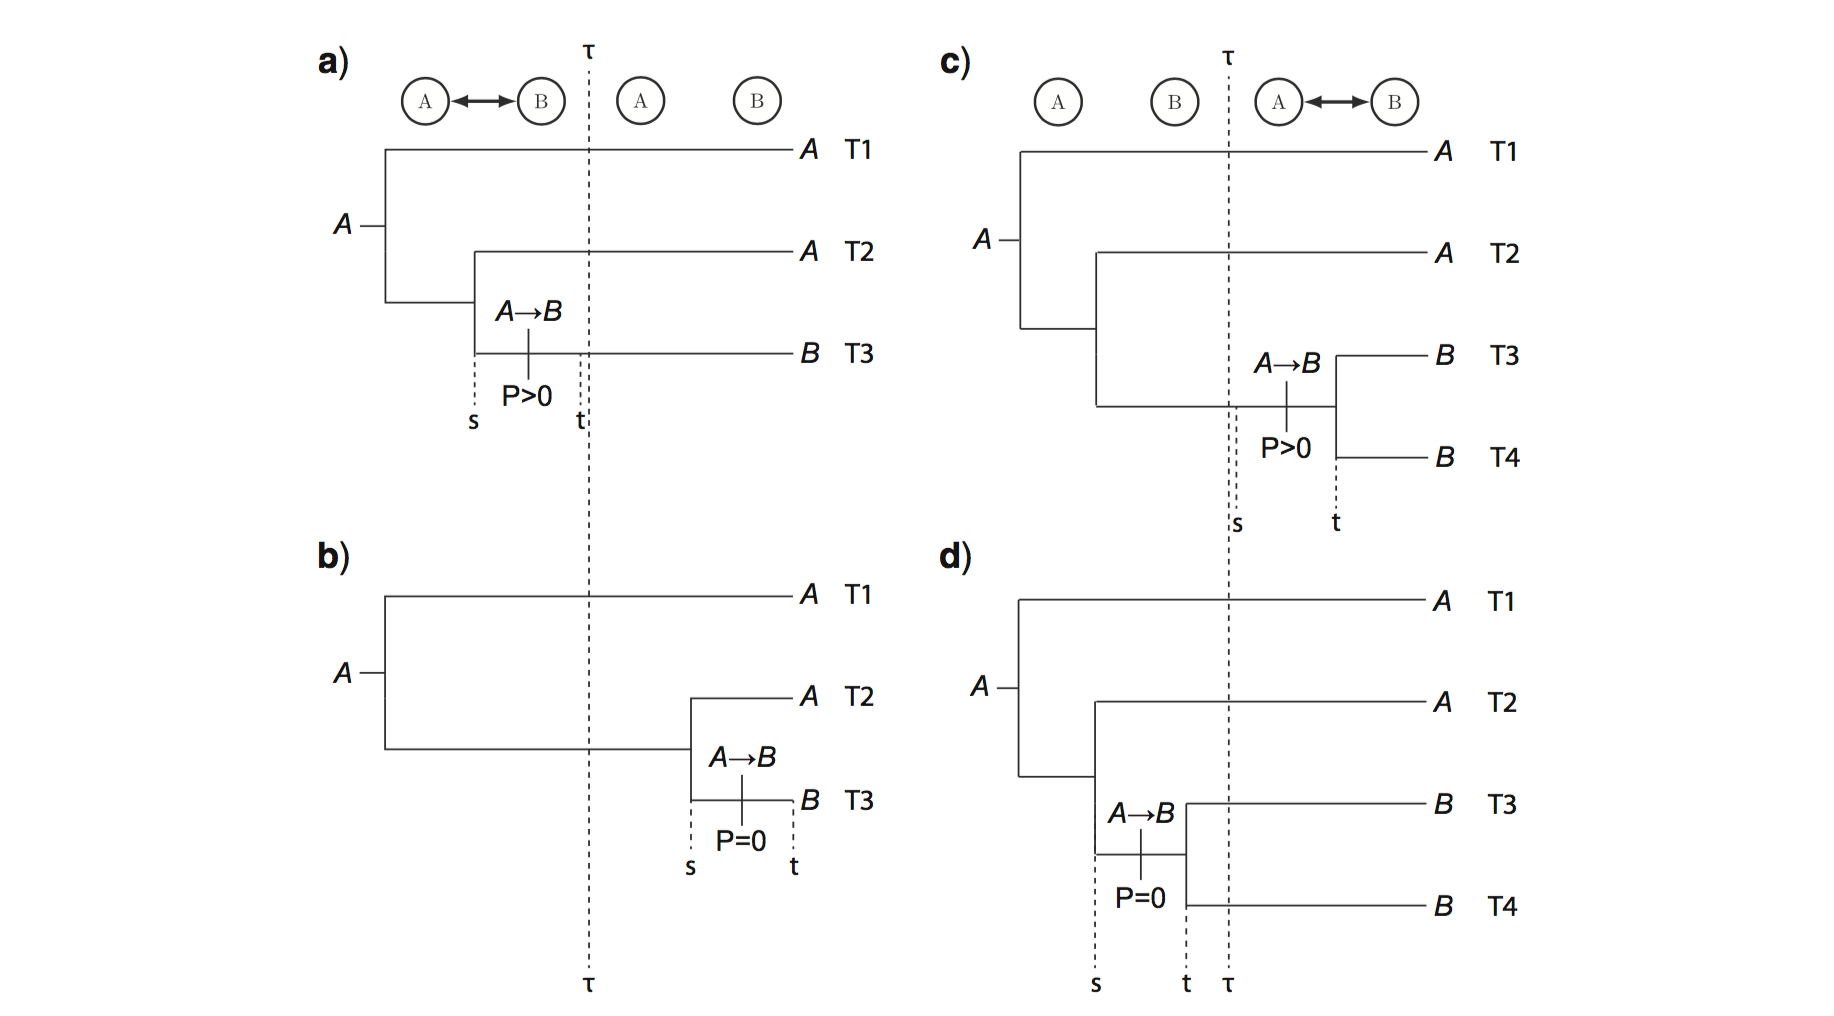
\includegraphics[width=\textwidth]{figures/fig_biogeo_dating.png}
\caption{Cartoon of biogeographic transition probabilities as functions of geological time, and how that relates to speciation times. (a) Areas split, dispersal before split, positive probability; (b) Areas split, dispersal after split, zero probability; (c) Areas merge, dispersal after merge, positive probability; (d) Areas merge, dispersal before merge, zero probabilty. [ Improve description later. ]}
\end{figure}

We will move from our simpler 4-area model to a 6-area model, where we now include the remaining Hawaiian islands (R) and the North American mainland (Z).
Additionally, we will add three tarweed taxa to our dataset, increasing the total number of taxa to 38.
We'll use internal transcribed spacer (ITS) to estimate the phylogeny, which is a 600 bp non-coding locus that is historically important for plant systematics.
Because the locus is relatively short, it will also leave us with a fair amount of phylogenetic uncertainty in branch length and topology estimates.
However, because we're estimating phylogeny and biogeography, it will be correctly incorporated into our ancestral range estimates.


Much of this tutorial will be similar to the previous section, except we are adding a birth-death process and a molecular substitution process to the model graph.

Create the necessary input/output variables.

\begin{snugshade}
\begin{lstlisting}
range_fn = "data/n6/silversword.n6.range.nex"
mol_fn   = "data/n6/silversword.mol.nex"
phy_fn   = "data/n6/silversword.tre"
out_fn   = "output/epoch_phy"
geo_fn   = "data/n6/hawaii.n6"
times_fn = geo_fn + ".times.txt"
dist_fn  = geo_fn + ".distances.txt"
\end{lstlisting}
\end{snugshade}

Add the analysis helper variables

\begin{snugshade}
\begin{lstlisting}
mvi = 1
mni = 1
n_gen = 1e5    # more parameters, longer run!
\end{lstlisting}
\end{snugshade}

% max range size

Impose limits to the maximum range size, both to prohibit widespread species ranges and to improve the computational efficiency of the method.

First, get the number of areas
\begin{snugshade}
\begin{lstlisting}
dat_range_01 = readDiscreteCharacterData(range_fn)
n_areas <- dat_range_01.nchar()
\end{lstlisting}
\end{snugshade}

Suppose we wanted to forbid ranges from being three or more areas in size.
The total number of ranges is $\sum_{k=0}^m {{n}\choose{k}}$ where $n$ is the total number of areas, $m$ is the maximum number of permissible areas, and ${{n}\choose{k}}$ is the number of ways to sample $k$ unordered areas from a pool of $n$ areas.

\begin{snugshade}
\begin{lstlisting}
max_areas <- 2
n_states <- 0
for (k in 0:max_areas) n_states += choose(n_areas, k)
\end{lstlisting}
\end{snugshade}

Then format the dataset for the reduced state space

\begin{snugshade}
\begin{lstlisting}
dat_range_n = formatDiscreteCharacterData(dat_range_01, "DEC", n_states)
\end{lstlisting}
\end{snugshade}


% read in some geography data

Read in the list of minimum and maximum ages of island formation

\begin{snugshade}
\begin{lstlisting}
time_bounds <- readDataDelimitedFile(file=times_fn, delimiter=" ")
n_epochs <- time_bounds.size()
\end{lstlisting}
\end{snugshade}

Read in a vector of matrices that describe the connectivity between areas over time.
Note, there is one connectivity matrix per epoch, ordered from oldest to youngest.

\begin{snugshade}
\begin{lstlisting}
for (i in 1:n_epochs) {
    connectivity[i] <- readDataDelimitedFile(file=geo_fn+"."+i+".txt", delimiter=" ")
}
\end{lstlisting}
\end{snugshade}

Read in the matrix of distances between all pairs of areas (km). For simplicity, we will assume that distances remain constant over time, even though they certainly vary.

\begin{snugshade}
\begin{lstlisting}
distances <- readDataDelimitedFile(file=dist_fn, delimiter=" ")
\end{lstlisting}
\end{snugshade}

\subsubsection{The tree model}

In this exercise we will also be estimating the phylogeny (topology and branch lengths), meaning our tree will be a stochastic node with a prior distribution.
For this, we'll use a constant rate birth-death process.

Assign root age with a maximum age of 15Ma to reflect the fossil pollen record for Californian tarweeds [cite].

\begin{snugshade}
\begin{lstlisting}
root_age ~ dnUniform(0, 15)
moves[mvi++] = mvScale(root_age, weight=2)
\end{lstlisting}
\end{snugshade}

Assign the proportion of sampled taxa (we have a non-uniform sampling scheme, but this should suffice).
\begin{snugshade}
\begin{lstlisting}
rho <- 35/50
\end{lstlisting}
\end{snugshade}

Assign the birth and death priors
\begin{snugshade}
\begin{lstlisting}
birth ~ dnExp(1)
moves[mvi++] = mvScale(birth)
death ~ dnExp(1)
moves[mvi++] = mvScale(death)
\end{lstlisting}
\end{snugshade}

Instantiate a tree variable generated by a birth-death process
\begin{snugshade}
\begin{lstlisting}
phy ~ dnBDP(lambda=birth, mu=death, rho=rho, rootAge=root_age, taxa=taxa)
\end{lstlisting}
\end{snugshade}


Add topology and branch length moves
\begin{snugshade}
\begin{lstlisting}
moves[mvi++] = mvNNI(phy, weight=n_branches/2)
moves[mvi++] = mvFNPR(phy, weight=n_branches/8)
moves[mvi++] = mvNodeTimeSlideUniform(phy, weight=n_branches/2)
\end{lstlisting}
\end{snugshade}

Provide a starting tree (improves mixing, not essential)

\begin{snugshade}
\begin{lstlisting}
phy.setValue(phy_init)
root_age.setValue(phy_init.rootAge())
\end{lstlisting}
\end{snugshade}


\subsubsection{The molecular model}

In addition, to inform our branch lengths (in relative time units) and our topology, we will specify a simple HKY+$\Gamma4$+UCLN model of molecular substitution.


First specify a base rate for the molecular clock. This prior is uniform over orders of magnitude, between $10^-6$ and $10^3$
\begin{snugshade}
\begin{lstlisting}
log10_rate_mol ~ dnUniform(-6, 3)
log10_rate_mol.setValue(-1)
moves[mvi++] = mvSlide(log10_rate_mol, weight=5, delta=0.2)
rate_mol := 10^log10_rate_mol
\end{lstlisting}
\end{snugshade}

Assign log-normal relaxed clock rate multipliers to each branch in the tree. These priors have a mean of 1 so each branch prefers a strict clock model in the absence of data.
\begin{snugshade}
\begin{lstlisting}
branch_sd <- 1.0
branch_mean <- 0.0 - 0.5 * branch_sd^2
for (i in 1:n_branches) {
    branch_rate_multiplier[i] ~ dnLognormal(mean=branch_mean, sd=branch_sd)
    moves[mvi++] = mvScale(branch_rate_multiplier[i])
    branch_rates[i] := rate_mol * branch_rate_multiplier[i]
}
\end{lstlisting}
\end{snugshade}

Now we'll create an HKY rate matrix. First the transition-transversion rate ratio (with prior with mean=1)

\begin{snugshade}
\begin{lstlisting}
kappa ~ dnGamma(2,2)
moves[mvi++] = mvScale(kappa)
\end{lstlisting}
\end{snugshade}

the base frequencies over A, C, G, and T

\begin{snugshade}
\begin{lstlisting}
bf ~ dnDirichlet([1,1,1,1])
moves[mvi++] = mvSimplexElementScale(bf, alpha=10, weight=2)
\end{lstlisting}
\end{snugshade}

then using the base frequencies and TsTv rate ratio to build the matrix

\begin{snugshade}
\begin{lstlisting}
Q_mol := fnHKY(kappa, bf)
\end{lstlisting}
\end{snugshade}

Next, we'll create a $+\Gamma4$ across site rate variation model.
This requires a parameter to control how much site rate heterogeneity there is.

\begin{snugshade}
\begin{lstlisting}
alpha ~ dnUniform(0,50)
moves[mvi++] = mvScale(alpha)
\end{lstlisting}
\end{snugshade}

and a discretized Gamma distribution with 4 categories

\begin{snugshade}
\begin{lstlisting}
site_rates := fnDiscretizeGamma(alpha, alpha, 4)
\end{lstlisting}
\end{snugshade}

When {\tt alpha} is large, then the Gamma distribution centers its density around the rate multiplier of 1, meaning that all sites evolve at similar rates.
When {\tt alpha} is small, the Gamma distribution presents more site rate heterogeneity.

Finally, we'll create our molecular model of substitution

\begin{snugshade}
\begin{lstlisting}
seq_mol ~ dnPhyloCTMC(Q=Q_mol, tree=phy, branchRates=branch_rates, siteRates=site_rates, type="DNA", nSites=dat_mol.nchar())
\end{lstlisting}
\end{snugshade}

and attach the ETS dataset

\begin{snugshade}
\begin{lstlisting}
seq_mol.clamp(dat_mol)
\end{lstlisting}
\end{snugshade}


\subsubsection{The biogeographic model}
% distances between areas

Dispersal rates might make use of some extrinsic information, such as geographical distances between areas \citep{macarthur67, webb12}.
We model this as $d_{ij} = a e ^ {-b g_{ij}}$ where $g_{ij}$ is the geographical distance between areas $i$ and $j$ and $a$ and $b$ are parameters that scale distance on linear and exponential scales, respectively. Note that all dispersal rates equal $a$ when $b=0$.

\begin{snugshade}
\begin{lstlisting}
dispersal_rate ~ dnExp(1)
dispersal_rate.setValue(0.1)
moves[mvi++] = mvScale(a)
b ~ dnUniform(-5,5)
b.setValue(0.01)
moves[mvi++] = mvSlide(b, delta=0.1)
\end{lstlisting}
\end{snugshade}

Now we can assign rates that are functions of distance between all pairs of areas

%dr[i][j][k] := (a * exp( -b * distances[j][k] ))
\begin{snugshade}
\begin{lstlisting}
for (i in 1:n_epochs) {
    for (j in 1:n_areas) {
        for (k in 1:n_areas) {
            dr[i][j][k] <- abs(0)
            if (connectivity[i][j][k] > 0) {
                dr[i][j][k] := a * exp( -b * distances[j][k] )
            }
        }
    }
}
\end{lstlisting}
\end{snugshade}


% extirpation penalized ranges
% ... they can exist, but not persist

It is unlikely that widespread ranges persist across disjunct areas for long periods of time.
Extirpation is more likely to occur in fragmented ranges than well-connected ranges, where peripheral populations are continuously reinforced from the center.

\begin{snugshade}
\begin{lstlisting}
e ~ dnExp(1)
moves[mvi++] = mvScale(e)

for (i in 1:n_epochs) {
    for (j in 1:n_areas) {
        for (k in 1:n_areas) {
            er[i][j][k] <- abs(0)
            if (j == k) {
                er[i][j][k] := e
            }
        }
    }
}

\end{lstlisting}
\end{snugshade}


% uncertainty in paleogeographic events

Treat epoch times as random variables. The present is always the present.
\begin{snugshade}
\begin{lstlisting}
for (i in 1:n_epochs) {
    time_max[i] <- time_bounds[i][1]
    time_min[i] <- time_bounds[i][2]
    if (i != n_epochs) {
        epoch_times[i] ~ dnUniform(time_min[i], time_max[i])
        moves[mvi++] = mvSlide(epoch_times[i], delta=0.5)
    } else {
        epoch_times[i] <- 0.0
    }
}
\end{lstlisting}
\end{snugshade}


% epoch model for anagenetic change

Build a rate matrix for each time interval
\begin{snugshade}
\begin{lstlisting}
for (i in 1:n_epochs) {
    Q[i] := fnDECRateMatrix(dispersalRates=connectivity[i],
                            extirpationRates=er,
                            maxRangeSize=max_areas)
}
\end{lstlisting}
\end{snugshade}


Create the epoch rate generator object
\begin{snugshade}
\begin{lstlisting}
Q_epoch := fnDECCladoProbs(
\end{lstlisting}
\end{snugshade}

% clado event probs

Here, we treat the probability of different types of cladogenetic events as a random variable to be estimate.

\begin{snugshade}
\begin{lstlisting}
clado_event_types <- [ "s", "a" ]
clado_type_probs ~ dnDirichlet( [1,1] )
moves[++mi] = mvSimplexElementScale(clado_type_probs, alpha=10)
P_clado := fnDECCladoProbs(eventProbs=clado_type_probs,
                           eventTypes=clado_event_types,
                           numCharacters=n_areas,
                           maxRangeSize=max_areas)
\end{lstlisting}
\end{snugshade}

For this dataset, we assume cladogenetic probabilities are constant with respect to geological time.


\begin{snugshade}
\begin{lstlisting}
rate_bg <- 1
\end{lstlisting}
\end{snugshade}


\begin{snugshade}
\begin{lstlisting}
rf_DEC <- rep(0, n_states)
rf_DEC[2] <- 1
rf_DEC <- simplex(rf_DEC)
\end{lstlisting}
\end{snugshade}


Create the phylogenetic model
\begin{snugshade}
\begin{lstlisting}
ctmc_bg ~ dnCTMCClado(tree=phy,
                      Q=Q_DEC_epoch,
                      cladoProbs=P_DEC,
                      branchRates=rate_bg,
                      rootFrequencies=rf_DEC,
                      type="NaturalNumbers",
                      nSites=1)
                  
\end{lstlisting}
\end{snugshade}


Attach the dataset
\begin{snugshade}
\begin{lstlisting}
ctmc_bg.clamp(dat_range_n)
\end{lstlisting}
\end{snugshade}


And the rest we've done before...
\begin{snugshade}
\begin{lstlisting}
# make the model
mdl = model(m)

# make the monitors
mn[1] = mnScreen(dispersal_rate, distance_scale, extirpation_rate, printgen=1000)
mn[2] = mnModel(file=out_fn+".params.txt", printgen=100)
mn[3] = mnJointConditionalAncestralState(tree=psi, ctmc=m, filename=out_fn+".states.txt", type="NaturalNumbers", printgen=100, withTips=true, withStartStates=true)

# make and run MCMC
ch = mcmc(mv,mn,mdl)
ch.burnin(1000, 10)
ch.run(10000)
\end{lstlisting}
\end{snugshade}


Finally, let's look at the trees and posterior distribution.

\begin{figure}[!ht]
\centering
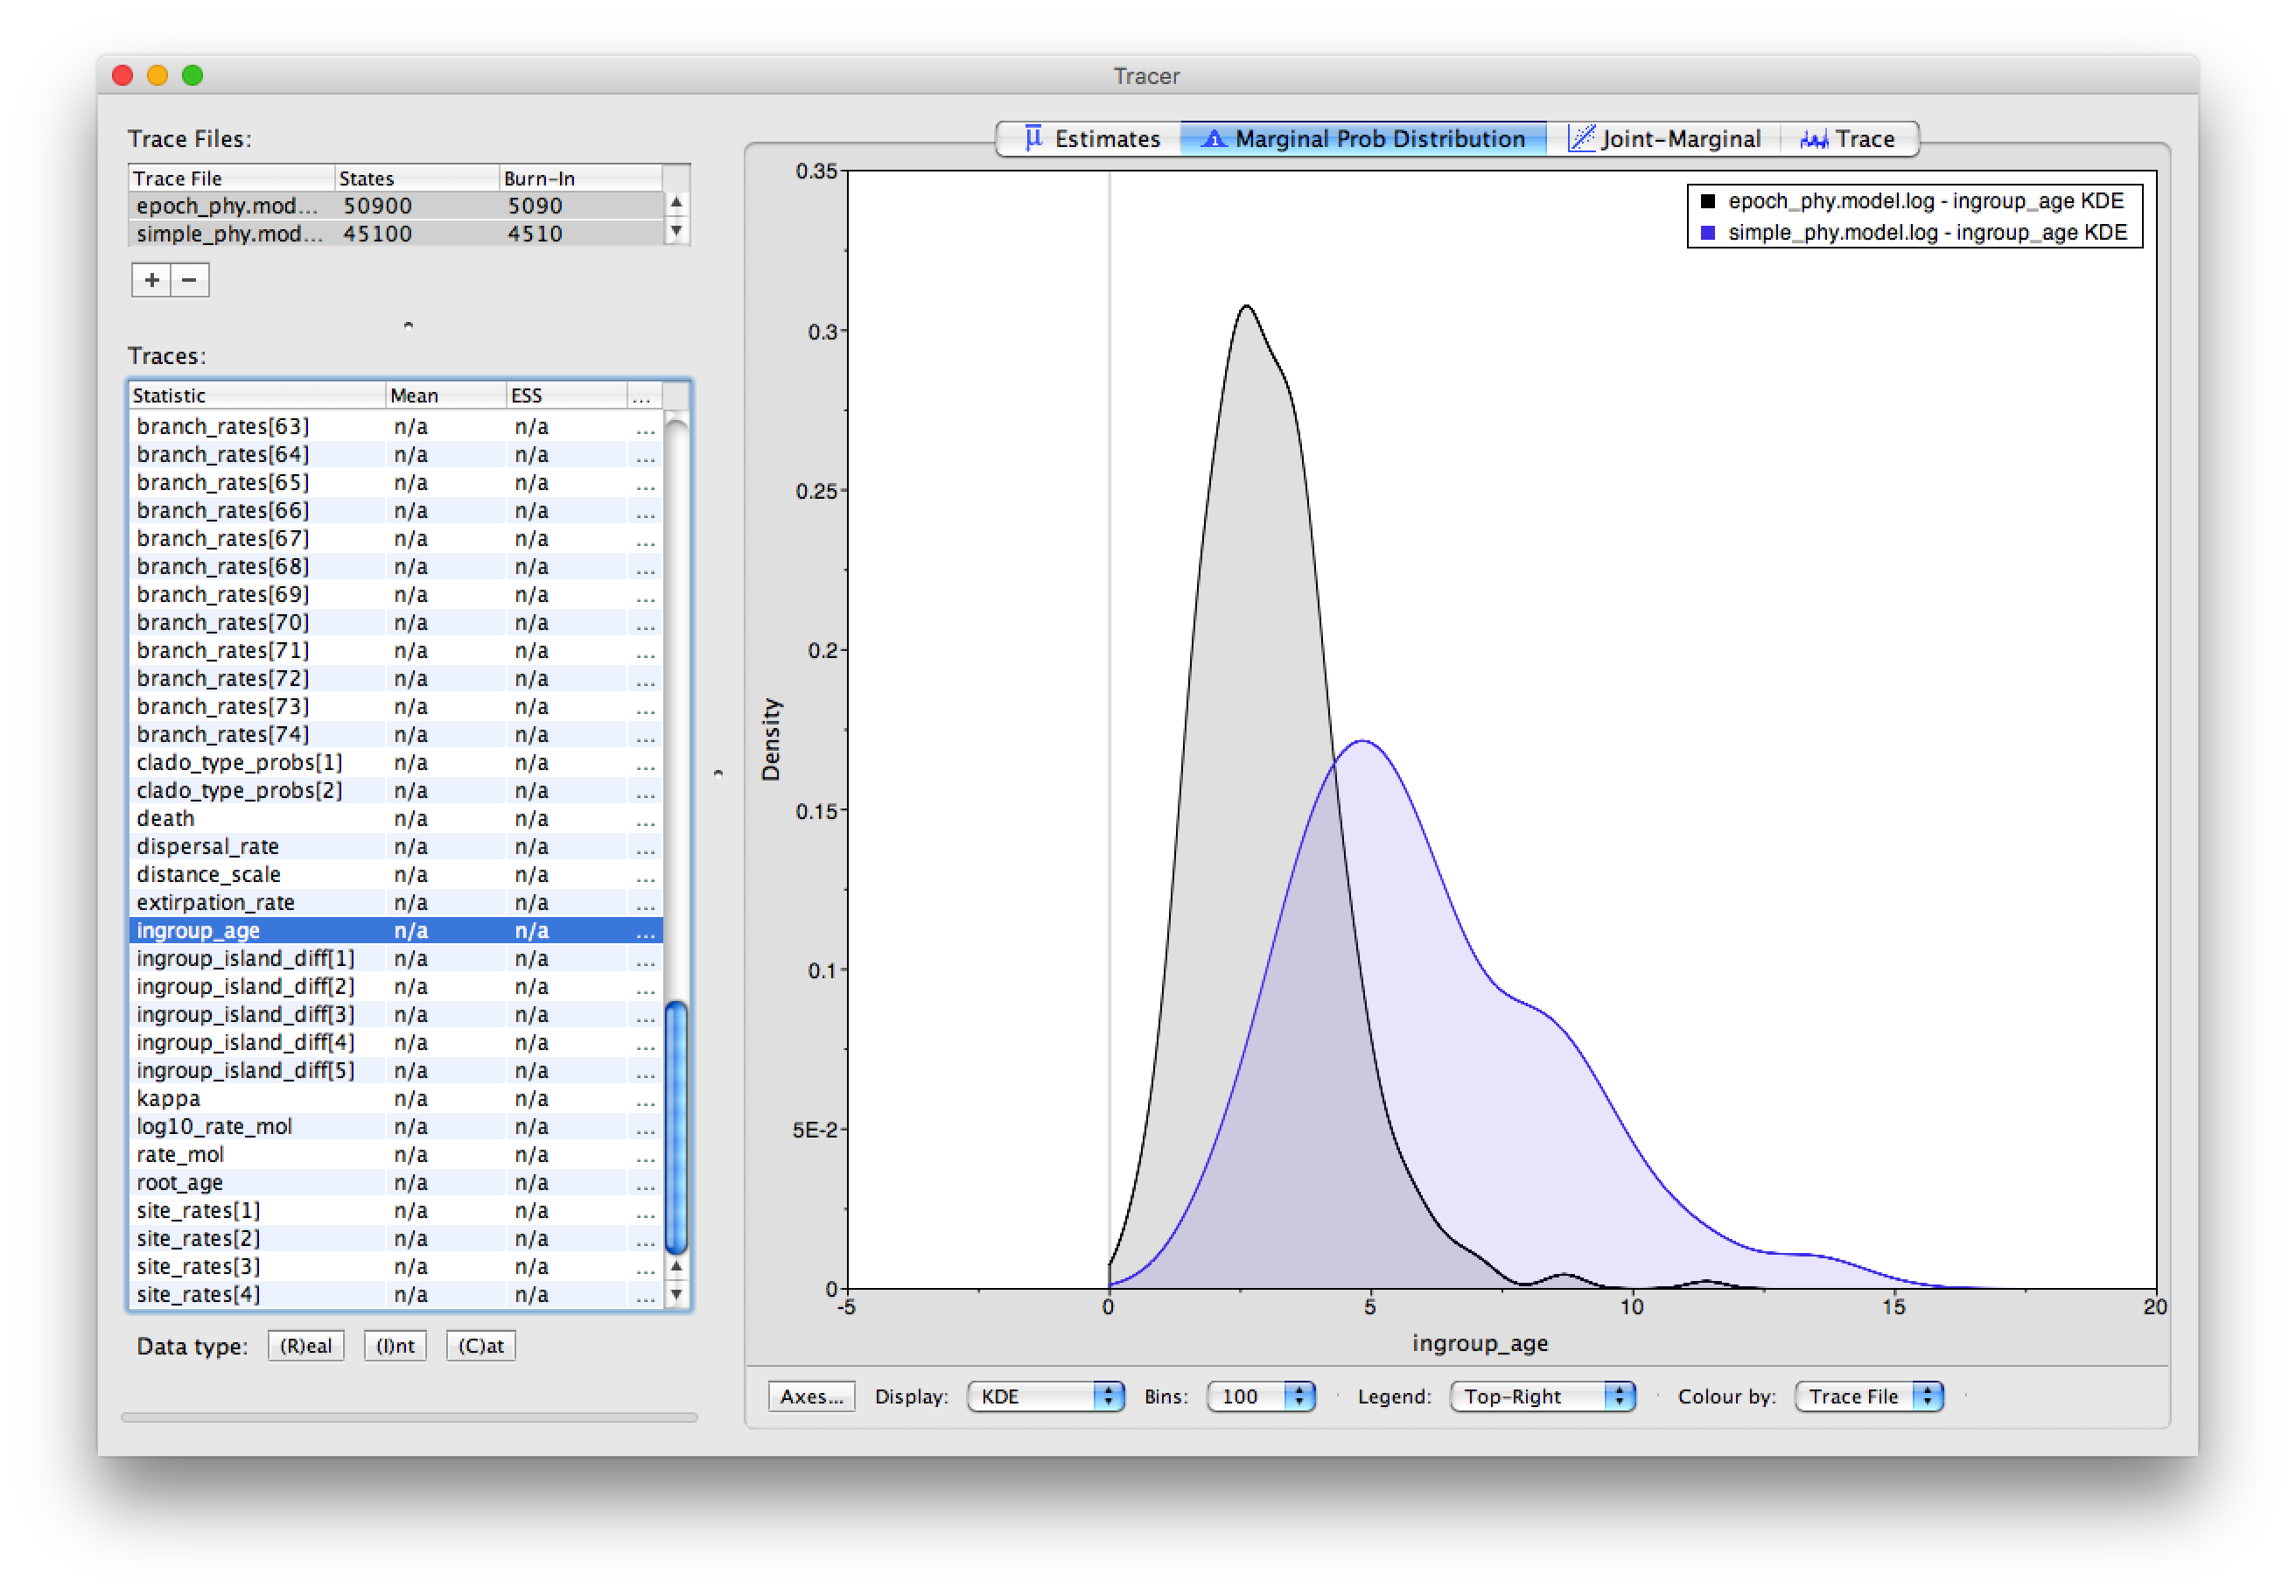
\includegraphics[width=0.7\textwidth]{figures/fig_biogeo_dating_ingroup_age.png}
\caption{Using the paleogeographic model largely prefers that silverswords originated after the formation of Kauai. Without paleogeography, silverswords originated as long as 15 Ma ago.}
\end{figure}


\begin{figure}[!ht]
\centering
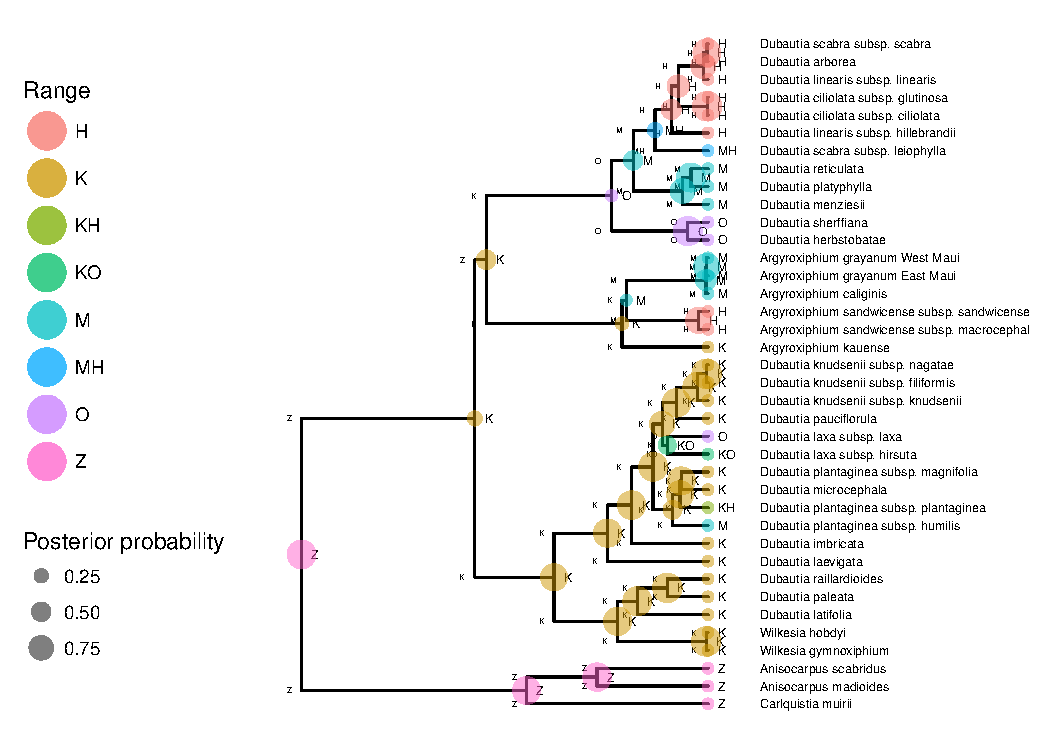
\includegraphics[width=0.7\textwidth]{figures/fig_epoch_phy_RevGadgets_ase.pdf}
\caption{Joint estimate of phylogeny and biogeography while incorporating paleogeographic information.}
\end{figure}



\begin{figure}[!ht]
\centering
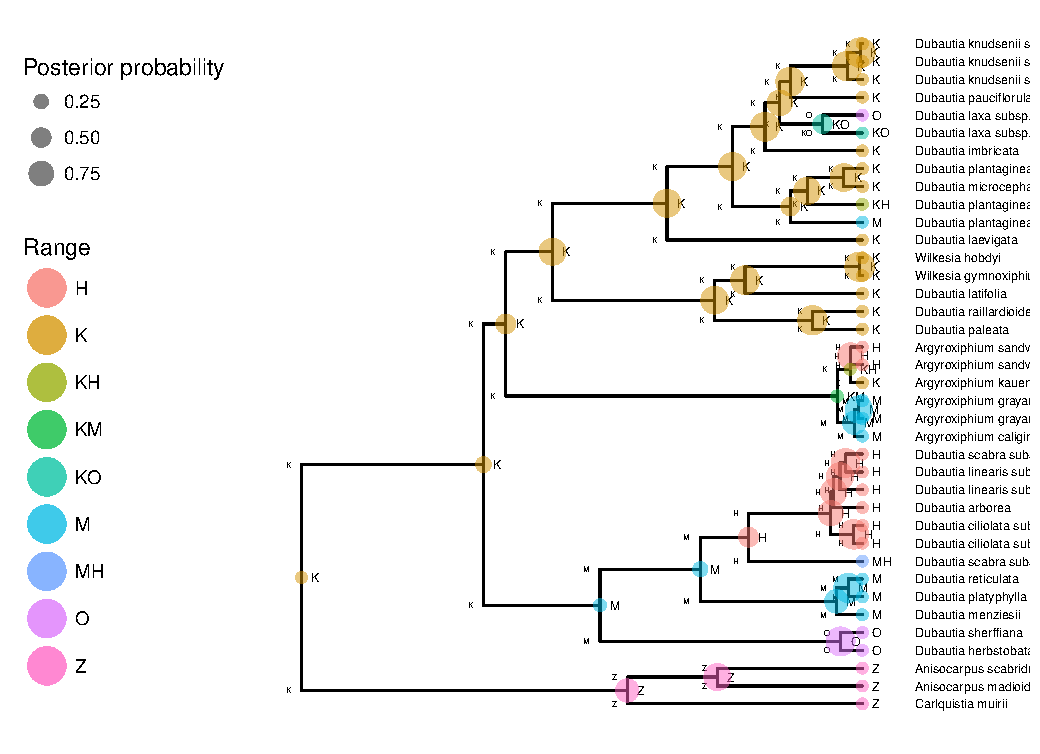
\includegraphics[width=0.7\textwidth]{figures/fig_simple_phy_RevGadgets_ase.pdf}
\caption{Joint estimate of phylogeny and biogeography ignoring paleogeographic information. This model has the tarweed+silversword clade originating in Kauai at a time when the island did not exist.}
\end{figure}



\newpage
